%version 1.00,	date 12/05/2016	auteur(s) Pierre Porche
\speaker{\Florian}

%%%%%%%% Slide MVC %%%%%%%%%%

\begin{frame}
  \frametitle{MV\underline{C} : Les contrôleurs}   
\begin{figure}[!h]
	\begin{center}
	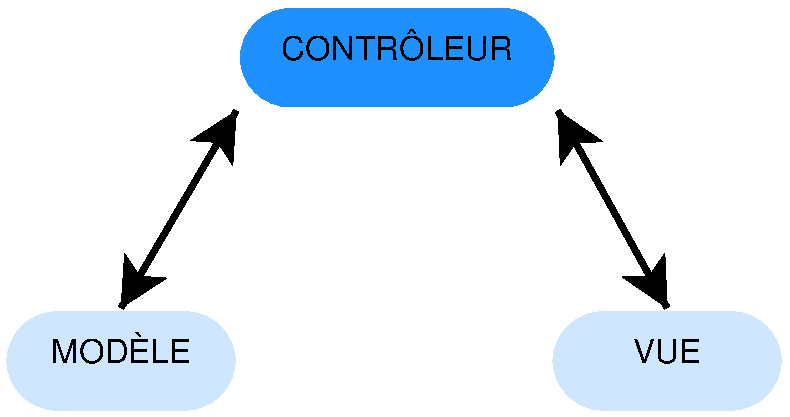
\includegraphics[scale=0.5]{images/mvcControleur}
	\caption{Architecture MV\underline{C}}
	\end{center}
\end{figure}
\end{frame}


%%%%%%%% Slide Bundle %%%%%%%%
\begin{frame}
  \frametitle{MV\underline{C} : Les contrôleurs}   
\begin{figure}[!h]
	\begin{center}
	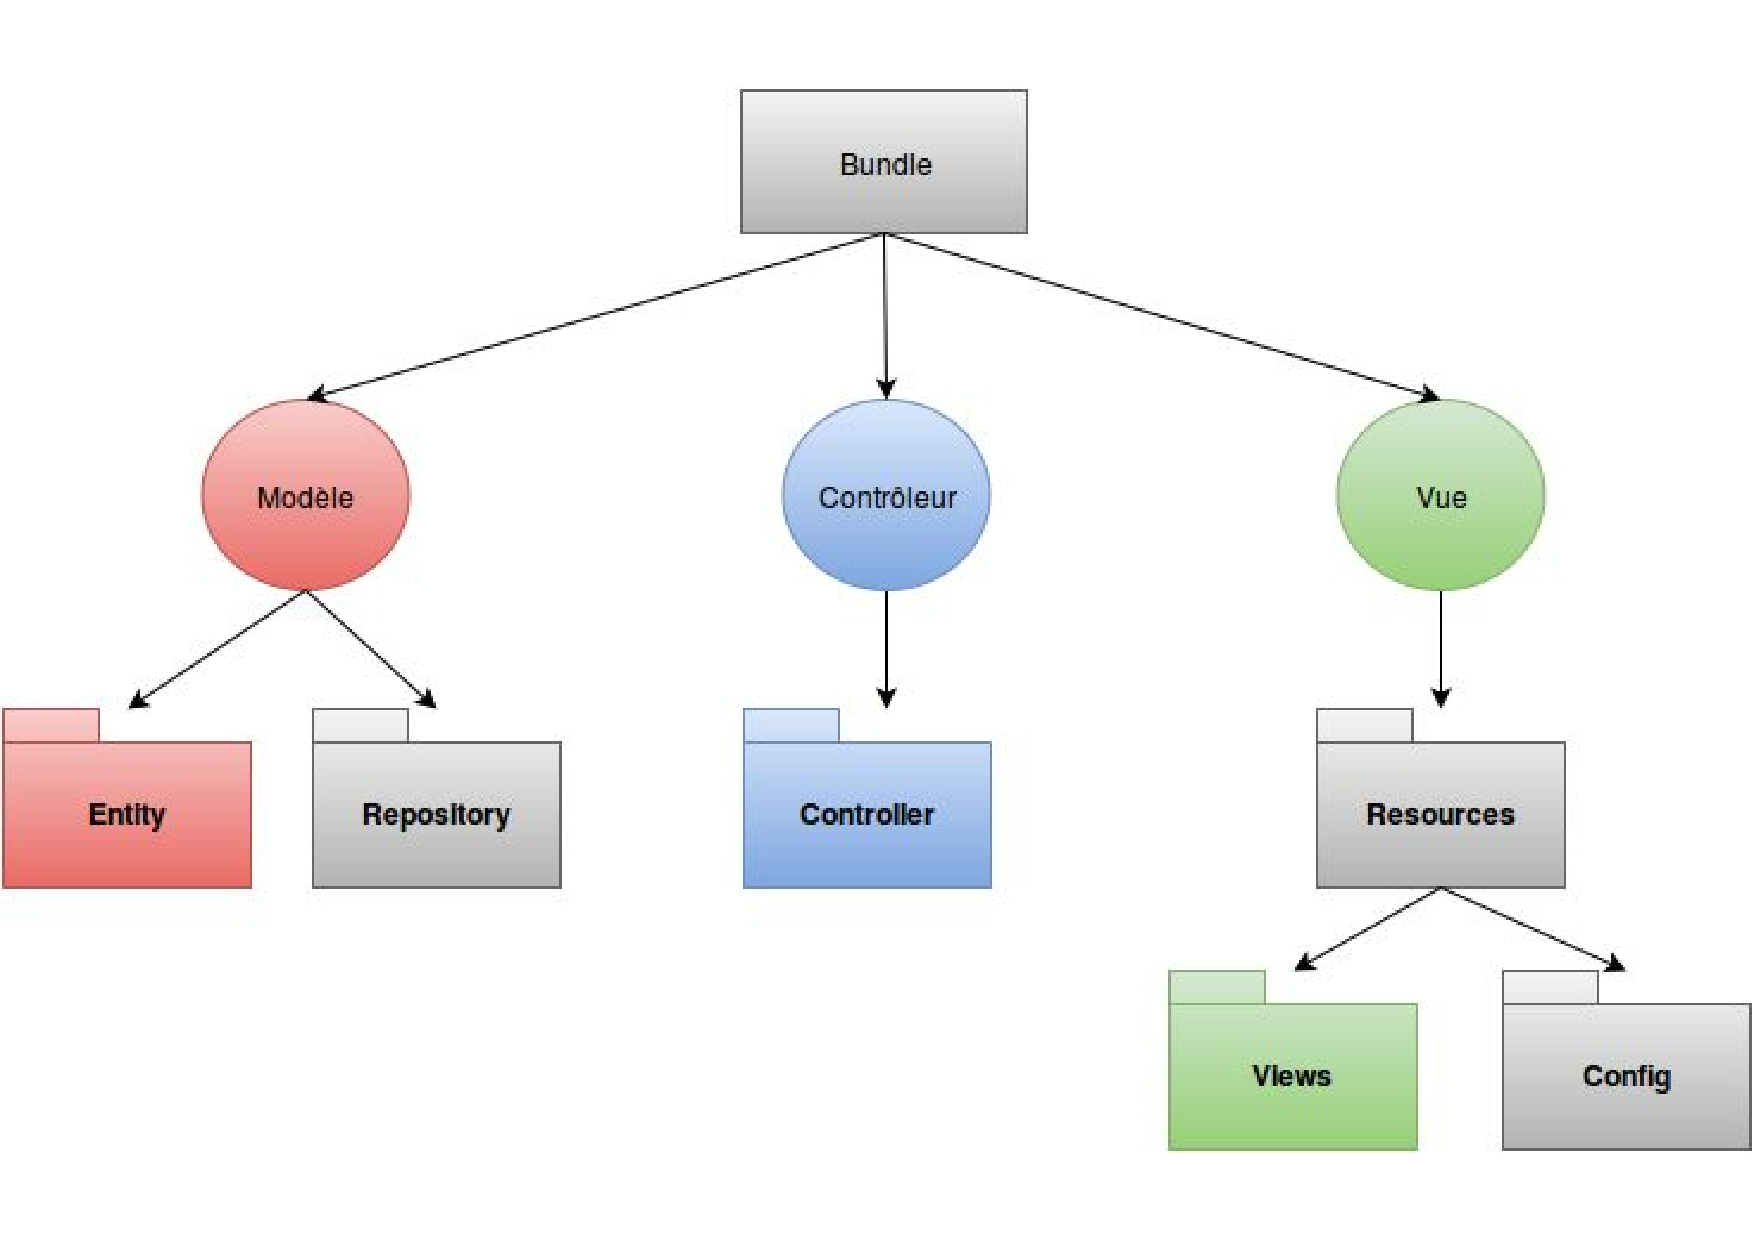
\includegraphics[scale=0.3]{images/bundles}
	\caption{Architecture d'un Bundle}
	\end{center}
\end{figure}
\end{frame}

%%%%%%%%%%% Slide fonctionnement %%%%%%%%

\begin{frame}
  \frametitle{MV\underline{C} : Les contrôleurs}
        \begin{figure}[!h]
	\begin{center}
	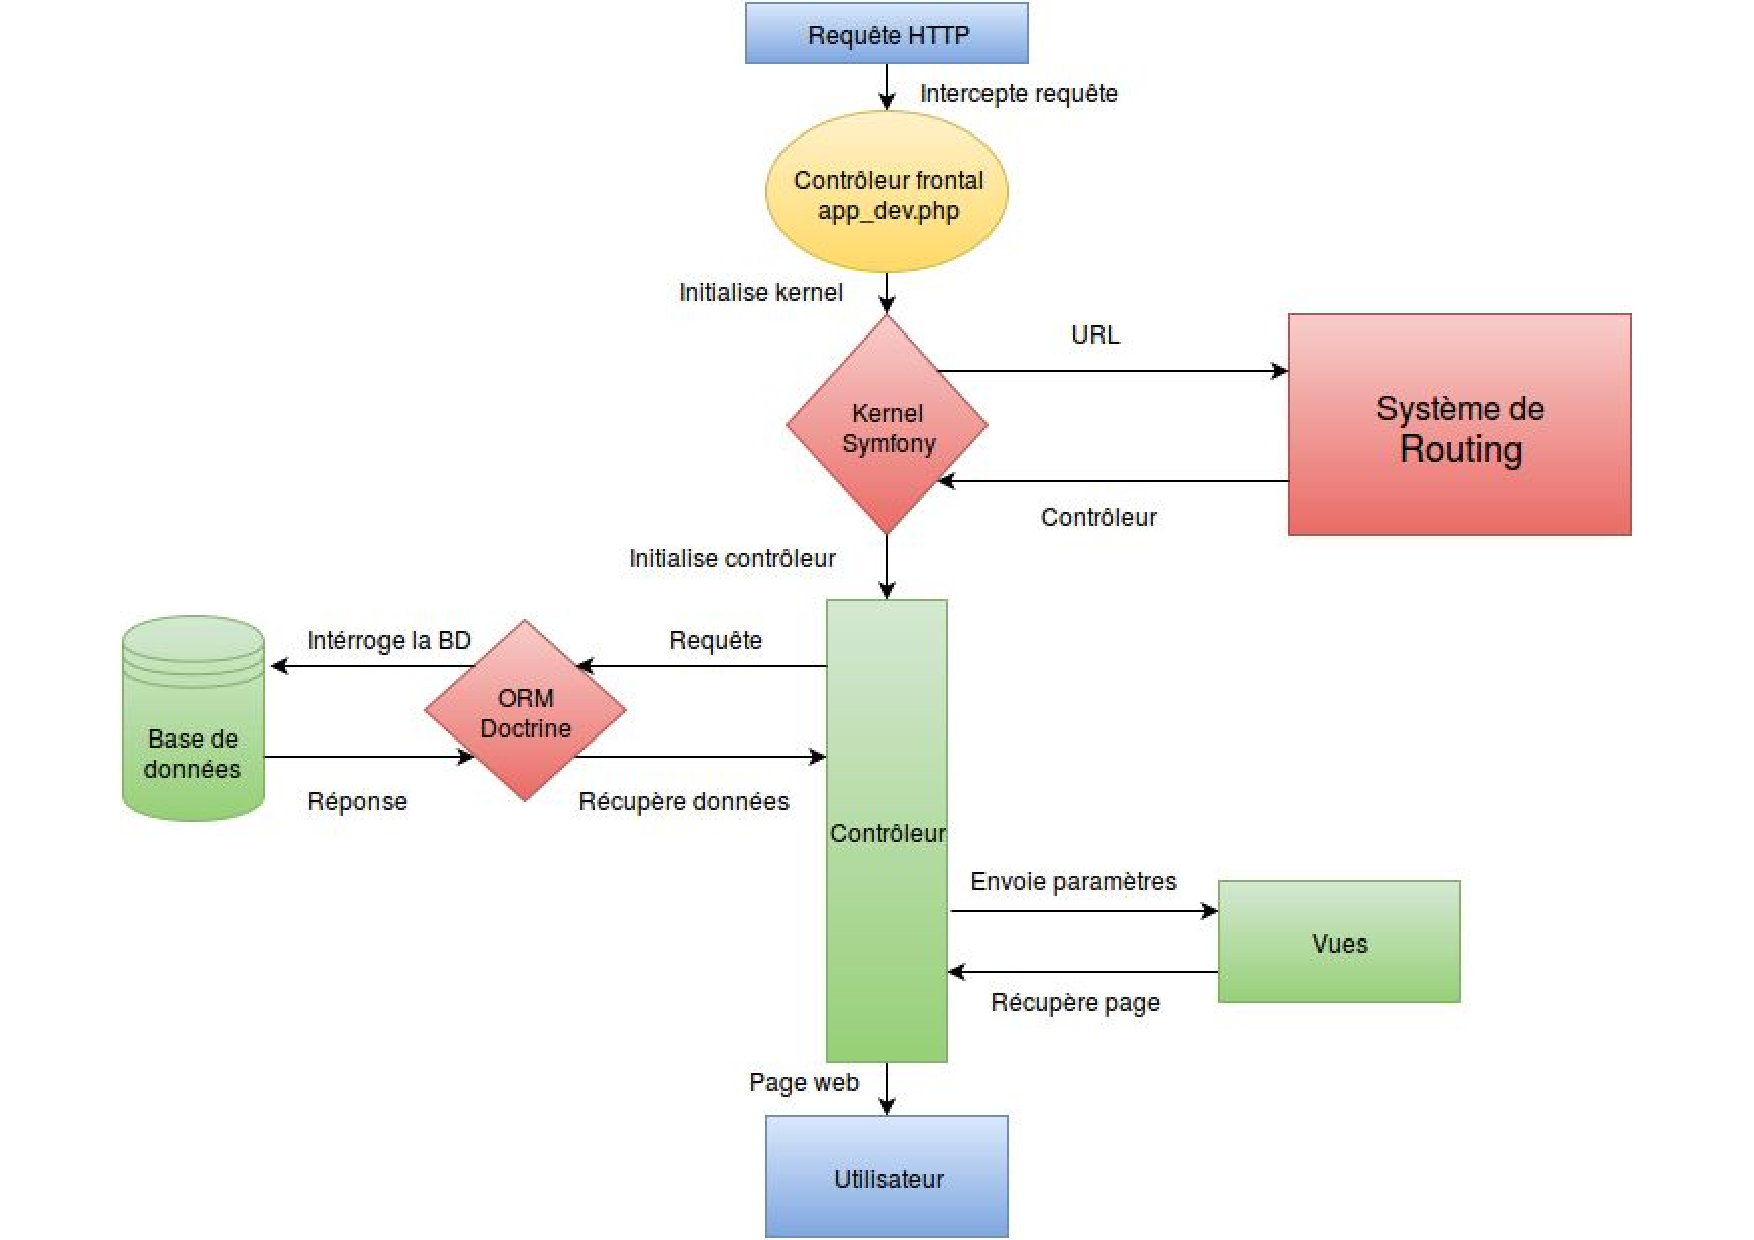
\includegraphics[scale=0.3]{images/symfony}
	\caption{Fonctionnement de l'application}
	\end{center}
\end{figure}
\end{frame}

%%%%%%%% Slide Nos Bundles %%%%%%%%%%

\begin{frame}
  \frametitle{MV\underline{C} : Les contrôleurs}
  \begin{block}{Notre architecture}
  \begin{itemize}
  \item Bundle Utilisateur : gestion des comptes utilisateur
  \item Bundle Intervention : gestion des interventions menées par les bénévoles
  \item Bundle Mail : gestion de l'envoi des emails
  \item Bundle Architecture : gestion de la structure de l'application
  \end{itemize}
  \end{block}   
  \end{frame}

%%%%%%%% Slide User Bundle %%%%%%

\begin{frame}
\begin{block}{Bundle Utilisateur}
\frametitle{MV\underline{C} : Les contrôleurs}
\begin{itemize}
\item Gestion des comptes utilisateurs
\item Création de compte
\item Envoi d'email contenant un lien d'activation
\item Mots de passe hashés et salés
\item Système d'authentification
\item Page de profil 
\end{itemize}
\end{block}
\end{frame}

%%%%%%%%%% Slide Architecture Bundle %%%%%%%

\begin{frame}
  \frametitle{MV\underline{C} : Les contrôleurs}
  \begin{block}{Bundle Architecture}
  \begin{itemize}
  \item Structure du projet	
  \item Pages d'accueil
  \item Page "à propos"
  \item Page "FAQ"
  \item Templates et thèmes
  \end{itemize}
  \end{block}   
  \end{frame}
